\chapter{Riemann Sums in Code and Practice}

\section{Code for a Riemann Sum}
\index{riemann sums!code}
You can create a program that automatically calculates a Riemann sum. Create a file called \filename{riemann.py} and type the following into it:

\begin{minted}{python}
import matplotlib.pyplot as plt
import sys
import math

from matplotlib.patches import Rectangle

# Did the user supply two arguments?
if len(sys.argv) != 3:
    print(f"Usage: {sys.argv[0]} <stop> <divisions>")
    print(f"Numerically integrates 1/x from 1 to <stop>.")
    print(f"Calculates the value of 1/x at <divisions> spots in the range.")
    exit(1)

# Check to make sure the number of divisions is greater than zero?
divisions = int(sys.argv[2])
if divisions <= 0:
    print("ERROR: Divisions must be at least 1.")
    exit(1)

# Is the stopping point after 1.0?
stop = float(sys.argv[1])
if stop <= 1.0:
    print("ERROR: Stopping point must be greater than 1.0")
    exit(1)

start = 1.0
step_size = (stop - start)/divisions

print(f"Step size is {step_size:.5f}.")
x_values = []
y_values = []
total = 0.0
for i in range(divisions):
    current_x = start + i * step_size
    current_y = 1.0/current_x
    area = current_y * step_size
    print(f"{i}: 1 / {current_x:.3f} = {current_y:4f}, area of rect = {area:8f} ")

    x_values.append(current_x)
    y_values.append(current_y)
    total += area
    print(f"\tCumulative={total:.3f}, ln({current_x:.3f})={math.log(current_x):.3f}")

print(f"Numerical integration of 1/x from 1.0 to {stop:.4f} is {total:.4f}")
print(f"The natural log of {stop:.4f} is {math.log(stop):.4f}")

# Create data for the smooth 1/x line
SMOOTH_DIVISIONS = 200
smooth_start = start - 0.15
smooth_stop = stop + 1.0
smooth_step = (smooth_stop - smooth_start)/SMOOTH_DIVISIONS
smooth_x_values = []
smooth_y_values = []
for i in range(SMOOTH_DIVISIONS):
    current_x = smooth_start + i * smooth_step
    current_y = 1.0/current_x
    smooth_x_values.append(current_x)
    smooth_y_values.append(current_y)

# Put it on a plot
fig, ax = plt.subplots()
ax.set_xlim((smooth_x_values[0], smooth_x_values[-1]))
ax.set_ylim((0, smooth_y_values[0]))
ax.set_title("Riemann Sums for 1/x")

# Make the Riemann rects
for i in range(divisions):
    current_x = x_values[i]
    next_x = current_x + step_size
    current_y = y_values[i]
    rect = Rectangle((current_x, 0), step_size, current_y, edgecolor="green", facecolor="lightgreen")
    ax.add_patch(rect)

# Make the true 1/x curve
ax.plot(smooth_x_values, smooth_y_values, c="k", label="1/x")

# Show the user
plt.show()

\end{minted}

This program will calculate and display a graph of the left Riemann sum of $\frac{1}{x}$ from 1 to the provided stop value with the indicated number of subintervals. When you run it, you will see a graph in a new window and something like this in the terminal:
\begin{minted}{python}
Step size is 0.40000.
0: 1 / 1.000 = 1.000000, area of rect = 0.400000 
	Cumulative=0.400, ln(1.000)=0.000
1: 1 / 1.400 = 0.714286, area of rect = 0.285714 
	Cumulative=0.686, ln(1.400)=0.336
2: 1 / 1.800 = 0.555556, area of rect = 0.222222 
	Cumulative=0.908, ln(1.800)=0.588
3: 1 / 2.200 = 0.454545, area of rect = 0.181818 
	Cumulative=1.090, ln(2.200)=0.788
4: 1 / 2.600 = 0.384615, area of rect = 0.153846 
	Cumulative=1.244, ln(2.600)=0.956
5: 1 / 3.000 = 0.333333, area of rect = 0.133333 
	Cumulative=1.377, ln(3.000)=1.099
6: 1 / 3.400 = 0.294118, area of rect = 0.117647 
	Cumulative=1.495, ln(3.400)=1.224
7: 1 / 3.800 = 0.263158, area of rect = 0.105263 
	Cumulative=1.600, ln(3.800)=1.335
8: 1 / 4.200 = 0.238095, area of rect = 0.095238 
	Cumulative=1.695, ln(4.200)=1.435
9: 1 / 4.600 = 0.217391, area of rect = 0.086957 
	Cumulative=1.782, ln(4.600)=1.526
Numerical integration of 1/x from 1.0 to 5.0000 is 1.7820
The natural log of 5.0000 is 1.6094
\end{minted}

\begin{Exercise}[label=rsumpython]
	Use the Python program you created to find $L_{10}$, $L_{50}$, $L_{100}$, $L_{500}$, $L_{1000}$, and $L_{5000}$ for the function $\frac{1}{x}$ from $x=1$ to $x=5$. What do you notice about the results?
\end{Exercise}

\begin{Answer}[ref=rsumpython]
	\begin{tabular}{c|c}
		Number of Intervals & Calculated Area \\
		10                  & 1.7820          \\
		50                  & 1.6419          \\
		100                 & 1.6256          \\
		500                 & 1.6126          \\
		1000                & 1.6110          \\
		5000                & 1.6098          \\
	\end{tabular}
	\\The area approaches the natural log of the endpoint, $\ln{5} \approx 1.6094$.
\end{Answer}

\section{Riemann Sum Practice}

\begin{Exercise}[label=rsum2]
	\begin{center}
		\begin{tabular}{c|c|c|c|c}
			t (hours)   & 4   & 7   & 12  & 15  \\
			R(t) (L/hr) & 6.5 & 6.2 & 5.9 & 5.6 \\
		\end{tabular}
	\end{center}
	A tank contains 50 liters of water after 4 hours of filling. Water is being added to the tank at rate $R(t)$. The value of $R(t)$ at select times is shown in the table. Using a right Riemann sum, estimate the amount of water in the tank after 15 hours of filling.
\end{Exercise}

\begin{Answer}[ref=rsum2]
	The volume of water will be the amount of water at 4 hours (50 liters) plus the area under the graph of $R(t)$ from $t=4$ to $t=15$. We will estimate this area with a right Riemann sum. The approximate volume added from $t=4$ to $t=7$ is $(7-4)*(6.2) = 18.6$ liters. The approximate volume added from $t=7$ to $t=12$ is $(12-7)*(5.9)=29.5$ liters. The approximate volume added from $t=12$ to $t=15$ is $(15-12)*(5.6) = 16.8$ liters. Therefore, the approximate total volume of water in the tank at $t=15$ is $50 + 18.6 + 29.5 + 16.8 = 114.9$ liters.
\end{Answer}

\begin{Exercise}[label=rsum3]
	Let $f(x) = x-2\ln{x}$. Estimate the area under $f$ from $x=1$ to $x=5$ using four rectangles and the value of $f$ at the midpoint of each interval. Sketch the curve and your approximating rectangles.
\end{Exercise}

\begin{Answer}[ref=rsum3]
	We will divide the area from $x=1$ to $x=5$ into four intervals at $x=2$, $x=3$, and $x=4$. Next, we will find the value of $f(x)$ at the midpoint of each interval:
	\begin{center}
		\begin{tabular}{c|c|c}
			Interval & Midpoint & Value of $f(x)$ at midpoint \\
			1        & 1.5      & $\approx0.68907$            \\
			2        & 2.5      & $\approx0.66742$            \\
			3        & 3.5      & $\approx0.99447$            \\
			4        & 4.5      & $\approx1.49185$            \\
		\end{tabular}
	\end{center}

	Using the values in the table, we can make a possible sketch of $f(x)$:\\
	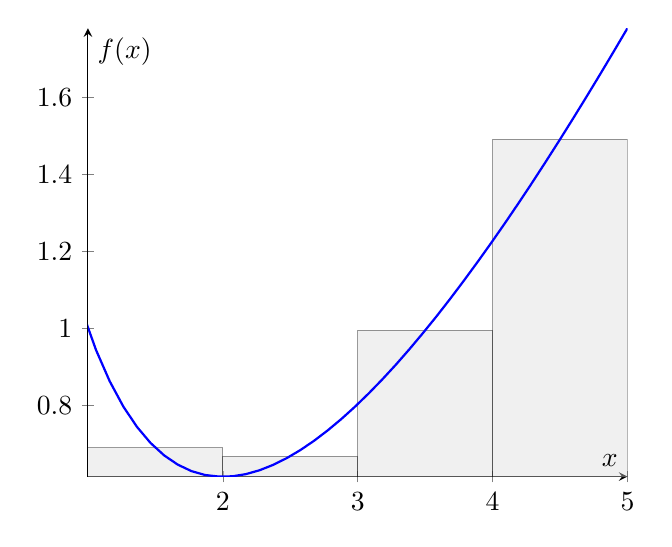
\begin{tikzpicture}
		\begin{axis}
			[axis lines = center, xmin=1, xmax=5, xlabel=$x$, ylabel=$f(x)$]
			\filldraw[fill=gray!30, draw=black, opacity=0.4](1,0) rectangle (2, 0.68907);
			\filldraw[fill=gray!30, draw=black, opacity=0.4](2, 0) rectangle (3, 0.66742);
			\filldraw[fill=gray!30, draw=black, opacity=0.4](3, 0) rectangle (4, 0.99447);
			\filldraw[fill=gray!30, draw=black, opacity=0.4](4, 0) rectangle (5, 1.49185);
			\addplot[blue, thick, samples=100]{x-2*ln(x)};
		\end{axis}
	\end{tikzpicture}\\
	And we calculate the total area in the rectangles:
	$$1\times(0.68907+0.66742+0.99447+1.49185)=3.84281$$
\end{Answer}

\begin{Exercise}[label=rsum4]
	A graph of a car's velocity over a period of 60 seconds is shown. Estimate the distance traveled during this period.
	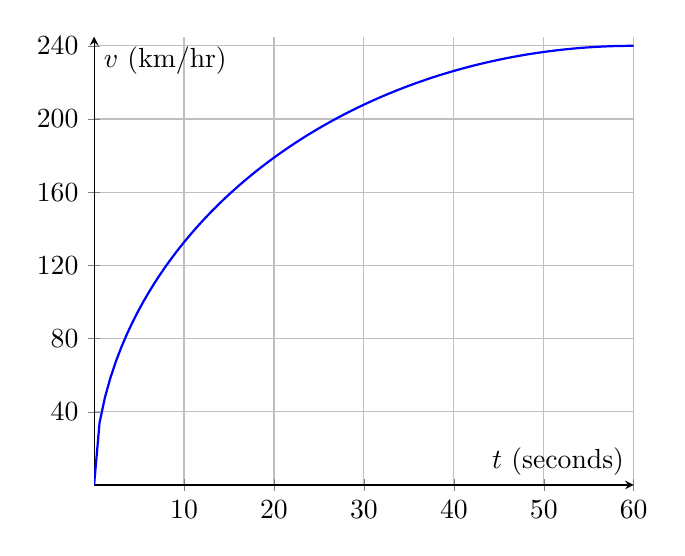
\begin{tikzpicture}
		\begin{axis}
			[axis lines = center,
				xmin = 0, xmax = 60, xlabel=$t$ (seconds),
				ymin=0, ymax=245, ylabel=$v$ (km/hr), ytick={40, 80, 120, 160, 200, 240}, xmajorgrids=true, ymajorgrids=true]
			\addplot[blue, thick, samples=100, domain=0:60]{4*sqrt(3600-(x-60)^2)};
		\end{axis}
	\end{tikzpicture}
\end{Exercise}

\begin{Answer}[ref=rsum4]
	The question allows the student to choose the type of sum (left, right, or midpoint) and the number of intervals. A possible solution is given, but there are many ways to answer the question.\\
	The tricky part here is noticing the units! The graph gives speed in km/hr but time in seconds, so we convert km/hr to m/s before multiplying (divide by 3.6). A possible solution is to divide the graph into 6 intervals (one every 10 seconds) and use a right Riemann sum.

	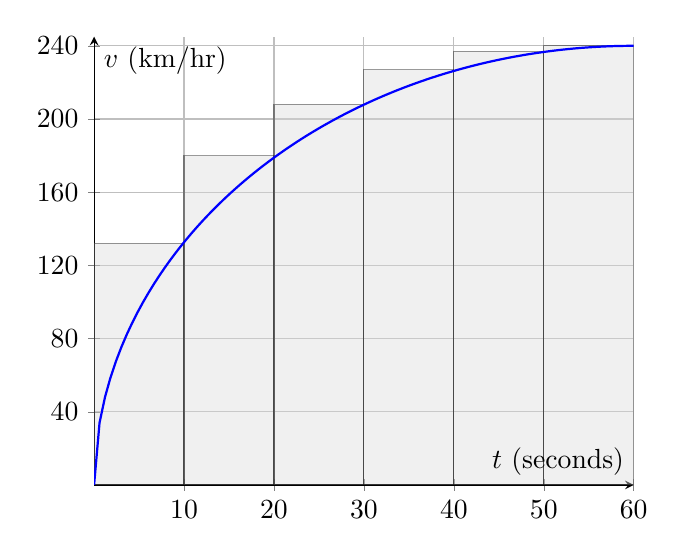
\begin{tikzpicture}
		\begin{axis}
			[axis lines = center,
				xmin = 0, xmax = 60, xlabel=$t$ (seconds),
				ymin=0, ymax=245, ylabel=$v$ (km/hr), ytick={40, 80, 120, 160, 200, 240}, xmajorgrids=true, ymajorgrids=true]
			\filldraw[fill=gray!30, draw=black, opacity=0.4](0,0) rectangle (10,132);
			\filldraw[fill=gray!30, draw=black, opacity=0.4](10, 0) rectangle (20, 180);
			\filldraw[fill=gray!30, draw=black, opacity=0.4](20, 0) rectangle (30, 208);
			\filldraw[fill=gray!30, draw=black, opacity=0.4](30, 0) rectangle (40, 227);
			\filldraw[fill=gray!30, draw=black, opacity=0.4](40, 0) rectangle (50, 237);
			\filldraw[fill=gray!30, draw=black, opacity=0.4](50, 0) rectangle (60, 240);
			\addplot[blue, thick, samples=100, domain=0:60]{4*sqrt(3600-(x-60)^2)};
		\end{axis}
	\end{tikzpicture}\\
	We can use the graph to \textit{estimate} the height of each rectangle. Some reasonable estimates are $f(10) = 130\frac{km}{hr}\approx36.1\frac{m}{s}$, $f(20) = 180\frac{km}{hr}=50\frac{m}{s}$, $f(30) = 210\frac{km}{hr}\approx58.3\frac{m}{s}$, $f(40) = 230\frac{km}{hr}\approx63.9\frac{m}{s}$, $f(50) = 235\frac{km}{hr}\approx65.3\frac{m}{s}$, and $f(60) = 240\frac{km}{hr}\approx66.7\frac{m}{s}$. [Any values within $\pm5$ of the listed values are reasonable.] Noting that each interval is $10$ sec wide and using the estimates of $f(x)$ listed, we can estimate that the distance traveled is $10\text{ }sec\times(36.1\frac{m}{s}+50\frac{m}{s}+58.3\frac{m}{s}+63.9\frac{m}{s}+65.3\frac{m}{s}+66.7\frac{m}{s})=3403$ meters, or about 3.4 km.
\end{Answer}
